\begin{name}
	{\tenchude}{ĐỀ ÔN TẬP SỐ 6}{LỚP TOÁN THẦY PHÁT}{\thoigian}
\end{name}
\setcounter{ex}{0}
\setcounter{bt}{0}
\Opensolutionfile{ans}[ans/ans-Vted-16-2023]
%%==========Câu 1
\begin{ex}%[2D4Y1-2]
\immini
{Điểm nào trong hình bên là điểm biểu diễn của số phức $z=2-i$?
\choice
{Điểm $P$}
{Điểm $Q$}
{Điểm $M$}
{\True Điểm $N$}}
{\begin{tikzpicture}[>=stealth,line join=round,line cap=round,font=\footnotesize,scale=1]
\draw[->] (-2.5,0)--(2.5,0)node[below]{$x$};
\draw[->] (0,-1.5)--(0,1.5)node[left]{$y$};
\fill (0,0)node[below left]{$O$} (-2,0)node[below left]{$-2$} (2,0)node[below right]{$2$} (0,-1)node[below left]{$-1$} (0,1)node[above left]{$1$};
\path (2,1)coordinate[label=above right:$M$](M) (2,-1)coordinate[label=below right:$N$](N) (-2,1)coordinate[label=above left:$P$](P) (-2,-1)coordinate[label=below left:$Q$](Q) ;
\foreach \diem in {M,N,P,Q} \fill[black](\diem)circle(1.5pt);
\draw[dashed] (M)--(N)--(Q)--(P)--(M);
\end{tikzpicture}}
\loigiai{
	Số phức $z=2-i$ được biểu diễn bởi điểm $N(2;-1)$.
}
\end{ex}

%%==========Câu 2
\begin{ex}%[2H3Y1-3]
Trong KG $Oxyz$, cho mặt cầu $(S)$ có tâm là gốc tọa độ $O$ và đi qua điểm $A(1; 2;-2)$. Bán kính của mặt cầu $(S)$ bằng
\choice
{$2$}
{\True $3$}
{$9$}
{$1$}
\loigiai{
	Bán kính của mặt cầu $R=OA=\sqrt{1^2+2^2+(-2)^2}=3$.
}
\end{ex}

%%==========Câu 3
\begin{ex}%[2D2Y5-1]
Nghiệm của phương trình $\log_{2}(x+8)=5$ là
\choice
{$x=17$}
{$x=2$}
{$x=40$}
{\True $x=24$}
\loigiai{
	Ta có $\log_{2}(x+8)=5 \Leftrightarrow x+8=2^5 \Leftrightarrow x=24$.
}
\end{ex}

%%==========Câu 4
\begin{ex}%[2H3Y2-2]
Trong KG $Oxyz$, cho mặt phẳng $(\alpha)\colon 2x-y-z+3=0$. Véc-tơ nào sau đây không là một véc-tơ pháp tuyến của $(\alpha)$?
\choice
{$\overrightarrow{n}_{4}=\left(1; \dfrac{-1}{2}; \dfrac{-1}{2}\right)$}
{$\overrightarrow{n}_{1}=(2;-1;-1)$}
{\True $\overrightarrow{n}_{3}=(6;-2;-3)$}
{$\overrightarrow{n}_{2}=(-2; 1; 1)$}
\loigiai{
	Véc-tơ không là một véc-tơ pháp tuyến của $(\alpha)$ là $\overrightarrow{n}_{3}=(6;-2;-3)$.
}
\end{ex}

%%==========Câu 5
\begin{ex}%[2D4Y1-1]
Phần ảo của số phức $z=2-3i$ bằng
\choice
{$-2$}
{\True $-3$}
{$3$}
{$2$}
\loigiai{
	Phần ảo của số phức $z=2-3i$ bằng $-3$.
}
\end{ex}

%%==========Câu 6
\begin{ex}%[2D3B2-1]
Cho $\displaystyle\int\limits_{1}^{2}2f(x)\mathrm{\,d}x=2$ và $\displaystyle\int\limits_{2}^{5}f(x)\mathrm{\,d}x=3$. Khi đó $\displaystyle\int\limits_{1}^{5}f(x)\mathrm{\,d}x$ bằng
\choice
{\True $4$}
{$2$}
{$5$}
{$6$}
\loigiai{
	Ta có $\displaystyle\int\limits_{1}^{2}2f(x)\mathrm{\,d}x=2 \Leftrightarrow \displaystyle\int\limits_{1}^{2}f(x)\mathrm{\,d}x=1$.\\
	Khi đó $\displaystyle\int\limits_{1}^{5}f(x)\mathrm{\,d}x=\displaystyle\int\limits_{1}^{2}f(x)\mathrm{\,d}x+\displaystyle\int\limits_{2}^{5}f(x)\mathrm{\,d}x=1+3=4$.
}
\end{ex}

%%==========Câu 7
\begin{ex}%[1D2Y2-1]
Một tổ gồm $10$ học sinh gồm $4$ nam $6$ nữ. Số cách chọn hai học sinh gồm cả nam và nữ là
\choice
{\True $\mathrm{C}_{4}^{1}\cdot \mathrm{C}_{6}^{1}$}
{$\mathrm{C}_{4}^{1}+\mathrm{C}_{6}^{1}$}
{$\mathrm{C}_{10}^{2}$}
{$\mathrm{A}_{10}^{2}$}
\loigiai{
	Số cách chọn hai học sinh gồm cả nam và nữ là $\mathrm{C}_{4}^{1}\cdot \mathrm{C}_{6}^{1}$.
}
\end{ex}

%%==========Câu 8
\begin{ex}%[2D1Y4-1]
Đồ thị hàm số $y=\dfrac{2x-3}{x-1}$ có các đường tiệm cận đứng và tiệm cận ngang lần lượt là
\choice
{$x=2$ và $y=1$}
{\True $x=1$ và $y=2$}
{$x=-1$ và $y=2$}
{$x=1$ và $y=-3$}
\loigiai{
	Đồ thị hàm số $y=\dfrac{2x-3}{x-1}$ có các đường tiệm cận đứng và tiệm cận ngang lần lượt là $x=1$ và $y=2$.
}
\end{ex}

%%==========Câu 9
\begin{ex}%[2D1Y1-2]
\immini
{Cho hàm số $f(x)$ bậc ba có đồ thị như hình vẽ. Hàm số đã cho đồng biến trên khoảng nào dưới đây?
\choice
{$(-\infty; 2)$}
{$(-2;+\infty)$}
{$(0; 2)$}
{\True $(2;+\infty)$}}
{\begin{tikzpicture}[x=1cm,y=1cm,scale=1,>=stealth]
		\def\aa{1} \def\bb{-3} \def\cc{0} \def\dd{2}
		\draw[->] (-1.5,0)--(3.5,0)node[below right]{$x$};
		\draw[->] (0,-2.3)--(0,2.7)node[left]{$y$};
		\fill (0,0)node[below left]{$O$};
		\draw[black,samples=150,smooth,domain=-1:3] plot(\x,{\aa*(\x)^3+\bb*(\x)^2+\cc*\x+\dd});
		\path (0,2)coordinate[label=above left:$2$](A) (2,0)coordinate[label=above:$2$](B) (0,-2)coordinate[label=left:$-2$](C) ;
		\foreach \diem in {A,B,C} \fill[black](\diem)circle(1pt);
		\draw[dashed] (2,0)--(2,-2)--(0,-2);
\end{tikzpicture}}
\loigiai{
Dựa vào đồ thị hàm số, ta có hàm số đồng biến trên $(2;+\infty)$.
}
\end{ex}

%%==========Câu 10
\begin{ex}%[2H1Y3-2]
Cho khối lăng trụ có chiều cao bằng $3a$, diện tích mặt đáy bằng $4a^{2}$. Thể tích của khối lăng trụ đó là
\choice
{\True $12a^{3}$}
{$4a^{3}$}
{$12a^{2}$}
{$4a^{2}$}
\loigiai{
	Thể tích của khối lăng trụ là $V=4a^{2}\cdot 3a=12a^{3}$.
}
\end{ex}

%%==========Câu 11
\begin{ex}%[2D4Y2-1]
	Cho số phức $z=2-3i$. Mô đun của số phức $w=(1+i)z$ là
	\choice
	{$|w|=\sqrt{37}$}
	{$|w|=4$}
	{\True$|w|=\sqrt{26}$}
	{$|w|=5$}
	\loigiai{
		Ta có $w=(1+i)z=5-i \Rightarrow |w|=\sqrt{26}$.
	}
\end{ex}

%%==========Câu 12
\begin{ex}%[2H2B1-2]
	Cho hình trụ có bán kính đáy bằng $r$, chiều cao bằng $h$. Biết rằng hình trụ đó có diện tích toàn phần gấp đôi diện tích xung quanh. Mệnh đề nào sau đây đúng?
	\choice
	{$h=\sqrt{2}r$}
	{$h=2r$}
	{\True$r=h$}
	{$r=2h$}
	\loigiai{
		Diện tích xung quanh của hình trụ là $S_{xq}=2\pi rh$.\\
		Diện tích toàn phần của hình trụ là $S_{tp}=S_{xq}+2S_{\text{đ}}=2\pi rh+2\pi r^2$.\\
		Theo giả thiết ta có $S_{\text{tp}}=2S_{xq} \Leftrightarrow 2\pi rh+2\pi r^2=4 \pi rh \Leftrightarrow 2\pi r^2=2 \pi rh \Leftrightarrow r=h$.
	}
\end{ex}

%%==========Câu 13
\begin{ex}%[2D3Y1-1]
	Họ nguyên hàm của hàm số $f(x)=\mathrm{e}^{2x}$ là
	\choice
	{$2\mathrm{e}^{2x}+C$}
	{$2x\mathrm{e}^{2x}+C$}
	{\True$\dfrac{1}{2}\mathrm{e}^{2x}+C$}
	{$\dfrac{1}{2}\mathrm{e}^{x}+C$}
	\loigiai{
		Ta có $\displaystyle\int \mathrm{e}^{2x} \mathrm{\,d}x=\dfrac{1}{2}\mathrm{e}^{2x}+C$.
	}
\end{ex}

%%==========Câu 14
\begin{ex}%[2D1Y5-7]
	Đồ thị hàm số $y=x^3-3x^2+5x-4$ đi qua điểm nào dưới đây?
	\choice
	{\True$Q(0;-4)$}
	{$N(-4;0)$}
	{$M(0;4)$}
	{$P(-1;1)$}
	\loigiai{
		\begin{enumerate}[*]
			\item Ta có $y(0)=-4$ suy ra đồ thị hàm số $y=x^3-3x^2+5x-4$ đi qua điểm $Q(0;-4)$.
			\item Ta có $y(-4)=-136$ suy ra đồ thị hàm số $y=x^3-3x^2+5x-4$ không đi qua điểm $N(-4;0)$.
			\item Ta có $y(0)=-4$ suy ra đồ thị hàm số $y=x^3-3x^2+5x-4$ không đi qua điểm $M(0;4)$.
			\item Ta có $y(-1)=-13$ suy ra đồ thị hàm số $y=x^3-3x^2+5x-4$ không đi qua điểm $P(-1;1)$.
		\end{enumerate}
	}
\end{ex}

%%==========Câu 15
\begin{ex}%[2D2Y4-2]
	Trên khoảng $(0;+\infty)$, hàm số $y=\log_3x$ có đạo hàm là
	\choice
	{$y'=\dfrac{x}{\ln 3}$}
	{$y'=x\ln 3$}
	{\True$y'=\dfrac{1}{x\ln 3}$}
	{$y'=\dfrac{\ln 3}{x}$}
	\loigiai{
		Ta có $y'=\dfrac{1}{x\ln 3}$.
	}
\end{ex}

%%==========Câu 16
\begin{ex}%[2D4Y2-1]
	Cho các số phức $z_1=3-2i$ và $z_2=-5+4i$, khi đó $z_1+z_2$ bằng
	\choice
	{$-8+6i$}
	{$2-2i$}
	{$8-6i$}
	{\True$-2+2i$}
	\loigiai{
		Ta có $z_1+z_2=-2+2i$.
	}
\end{ex}

%%==========Câu 17
\begin{ex}%[2D2Y6-1]
	Tập nghiệm của bất phương trình $4^x \ge 2$ là
	\choice
	{$\left(\dfrac{1}{4};+\infty\right)$}
	{$\left[\dfrac{1}{4};+\infty\right)$}
	{\True$\left[\dfrac{1}{2};+\infty\right)$}
	{$\left(\dfrac{1}{2};+\infty\right)$}
	\loigiai{
		$4^x \ge 2 \Leftrightarrow 2^{2x} \ge 2 \Leftrightarrow 2x \ge 1 \Leftrightarrow x \ge \dfrac{1}{2}$.\\
		Vậy tập nghiệm của bất phương trình là $S=\left[\dfrac{1}{2};+\infty\right)$.
	}
\end{ex}

%%==========Câu 18
\begin{ex}%[2H3Y3-1]
	Trong KG $Oxyz$, cho đường thẳng $d \colon \heva{&x=1+2t\\&y=2-t\\&z=3+t}$. Một véc-tơ chỉ phương của $d$ có tọa độ là
	\choice
	{$(2;1;1)$}
	{\True$(2;-1;1)$}
	{$(1;2;3)$}
	{$(2;0;0)$}
	\loigiai{
		Đường thẳng $d$ có một véc-tơ chỉ phương là $\vec{u}_{d}=(2;-1;1)$.
	}
\end{ex}

%%==========Câu 19
\begin{ex}%[2D2Y3-1]
	Với mọi số thực $a$ dương, $\log_3(3a^2)$ bằng
	\choice
	{\True$1+2\log_3a$}
	{$3\log_3a$}
	{$2+3\log_3a$}
	{$1+\log_3a$}
	\loigiai{
		Ta có $\log_3(3a^2)=\log_33+\log_3a^2=1+2\log_3a$.
	}
\end{ex}

%%==========Câu 20
\begin{ex}%[1D3Y4-3]
	Cho cấp số nhân $(u_n)$ với $u_1=5$ và công bội $q=6$. Giá trị của $u_2$ bằng
	\choice
	{$1$}
	{$11$}
	{$3$}
	{\True$30$}
	\loigiai{
		Ta có $u_2=qu_1=6\cdot5=30$.
	}
\end{ex}

%%==========Câu 21
\begin{ex}%[2H2B1-1]
	Đường kính của khối cầu có thể tích $36\pi a^3$ bằng
	\choice
	{$3a$}
	{$2a$}
	{\True $6a$}
	{$4a$}
	\loigiai{
		Ta có $V=\dfrac{4}{3}\pi R^3\Leftrightarrow R^3=\dfrac{3\cdot V}{4\pi}\Leftrightarrow R^3=\dfrac{3\cdot 36\pi a^3}{4\pi}=27a^3\Leftrightarrow R=3a$.\\
		Vậy đường kính khối cầu đã cho là $6a$.
	}
\end{ex}

%%==========Câu 22
\begin{ex}%[2H1Y3-2]
	Một khối chóp có diện tích đáy bằng $3\sqrt{2}$ và thể tích bằng $\sqrt{50}$. Chiều cao của khối chóp đó bằng
	\choice
	{$\dfrac{5}{3}$}
	{$10$}
	{\True $5$}
	{$\dfrac{10}{3}$}
	\loigiai{
		Ta có $V=\dfrac{1}{3}B\cdot h\Leftrightarrow h=\dfrac{3V}{B}=\dfrac{3\cdot \sqrt{50}}{3\sqrt{2}}=5.$
	}
\end{ex}

%%==========Câu 23
\begin{ex}%[2H3B3-2]
	Trong KG $Oxyz$, đường thẳng đi qua  $M\left(1;2;-1\right)$ đồng thời vuông góc mặt phẳng $2x+3y+4z+1=0$ có phương trình là
	\choice
	{\True $\dfrac{x-1}{2}=\dfrac{y-2}{3}=\dfrac{z+1}{4}$}
	{$\dfrac{x+2}{1}=\dfrac{y+3}{2}=\dfrac{z+4}{-1}$}
	{$\dfrac{x+1}{2}=\dfrac{y+2}{3}=\dfrac{z-1}{4}$}
	{$\dfrac{x-2}{1}=\dfrac{y-3}{2}=\dfrac{z-4}{-1}$}
	\loigiai{
		Vì $d \perp (P) \colon 2x+3y+4z+1=0$ nên vec-tơ chỉ phương của $d$ chính là vec-tơ pháp tuyến của $(P)$\\ hay $\vec{u}_d=\vec{n}_{(P)}=(2;3;4)$.\\
		Khi đó đường thẳng $d$ đi qua điểm $M$ nhận $\vec{n}_{(P)}=(2;3;4)$ làm vec-tơ chỉ phương có phương trình\\  $\dfrac{x-1}{2}=\dfrac{y-2}{3}=\dfrac{z+1}{4}$.
	}
\end{ex}

%%==========Câu 24
\begin{ex}%[2D1Y2-2]
	Cho hàm số $f(x)$ có bảng biến thiên
	\begin{center}
		\begin{tikzpicture}[font=\normalsize,t style/.style={style=solid}]
			\tkzTabInit[nocadre=true,lgt=1.2,espcl=2.5,deltacl=0.5]
			{$x$ /0.75, $f'(x)$/0.75, $f(x)$/1.75}
			{$-\infty $,$ 1 $,$ 5 $,$ +\infty$}
			\tkzTabLine{  , +,0 , -,0  , +,  }
			\path ($(N12)!0.9!(N13)$) node (A1){$-\infty$}
			($(N22)!0.2!(N23)$) node (A2){$3$}
			($(N32)!0.9!(N33)$) node (A3){$-5$}
			($(N42)!0.2!(N43)$) node (A4){$+\infty$};
			\foreach \x/\y in {A1/A2,A2/A3,A3/A4}{
				\draw[-stealth] (\x)--(\y);
			}
		\end{tikzpicture}
	\end{center}
	Giá trị cực đại của hàm số là
	\choice
	{$0$}
	{$1$}
	{$2$}
	{\True $3$}
	\loigiai{
		Dựa vào bảng biến thiên, ta có giá trị cực đại của hàm số là $3$.
	}
\end{ex}

%%==========Câu 25
\begin{ex}%[2H3B1-2]
	Trong KG $Oxyz$, cho vec-tơ $\vec{u}=\left(1;1;-2\right), \vec{v}=\left(1;0;2+\sqrt{6}\right)$. Góc giữa hai vec-tơ đã cho bằng
	\choice
	{$45^\circ$}
	{$120^\circ$}
	{\True $135^\circ$}
	{$60^\circ$}
	\loigiai{
		Gọi $\varphi$ là góc giữa hai vec-tơ $\vec{u}, \vec{v}$.\\
		Ta có $\cos \varphi=\dfrac{\vec{u}\cdot \vec{v}}{\left.|\vec{u}\right|\cdot \left.|\vec{v}\right|}=\dfrac{1\cdot 1+1\cdot 0-2\cdot \left(2+\sqrt{6}\right)}{\sqrt{1^2+1^2+(-2)^2}\cdot \sqrt{1^2+0^2+\left(2+\sqrt{6}\right)^2}}=-\dfrac{\sqrt{2}}{2}\Rightarrow\varphi=135^\circ$.
	}
\end{ex}

%%==========Câu 26
\begin{ex}%[2D2Y2-1]
	Tập xác định của hàm số $y=x^{\frac{1}{3}}+\left(x-1\right)^{-3}$ là
	\choice
	{$\mathbb{R}\backslash \left\{1\right\}$}
	{$\left(0;1\right)$}
	{\True $\left(0;+\infty\right)\backslash \left\{1\right\}$}
	{$\left(0;+\infty\right)$}
	\loigiai{
		Hàm số xác định khi và chỉ khi $\heva{&x>0\\&x-1\ne 0}\Leftrightarrow\heva{&x>0\\&x\ne 1.}$\\
		Vậy tập xác định $\mathscr{D}=\left(0;1\right)\backslash \left\{1\right\}$.
	}
\end{ex}

%%==========Câu 27
\begin{ex}%[2D1B1-1]
	Hàm số nào dưới đây nghịch biến trên $\mathbb{R}$?
	\choice
	{$y=x^4-1$}
	{\True $y=-x^3+x^2-5x$}
	{$y=\dfrac{x+3}{3x-1}$}
	{$y=x^2+3x+2$}
	\loigiai{
		Hàm số nghịch biến trên $\mathbb{R}$ thì 
		\begin{itemize}
			\item Tập xác định của nó phải là $\mathbb{R}\Rightarrow$ loại C.
			\item Đạo hàm $y'\le 0,\forall x\in \mathbb{R}$.
		\end{itemize}
		với phương án C, ta có $y'=-3x^2+4x-4\le 0, \forall x$
	}
\end{ex}

%%==========Câu 28
\begin{ex}%[2D3Y1-1]
	Nếu $\displaystyle\int\limits_2^3{f(x)\mathrm{d}x}=3$ và $\displaystyle\int\limits_2^3{\left[f(x)+g(x)\right]\mathrm{d}x}=1$ thì $\displaystyle\int\limits_2^3{g(x)\mathrm{d}x}$ bằng
	\choice
	{$4$}
	{\True $-2$}
	{$2$}
	{$3$}
	\loigiai{
		Ta có $\displaystyle\int\limits_2^3{\left[f(x)+g(x)\right]\mathrm{d}x}=1\Leftrightarrow \displaystyle\int\limits_2^3{f(x)\mathrm{d}x}+\displaystyle\int\limits_2^3{g(x)\mathrm{d}x}=1\Leftrightarrow \displaystyle\int\limits_2^3{g(x)\mathrm{d}x}=1-\displaystyle\int\limits_2^3{f(x)\mathrm{d}x}=-2$.
	}
\end{ex}

%%==========Câu 29
\begin{ex}%[2D1B2-2]
	\immini{Cho hàm số $y=ax^4+bx^2+cx+d,\,\, \left(a,b,c,d\in \mathbb{R}\right)$. Hàm số $y=f'(x)$ có đồ thị như hình vẽ. Số điểm cực trị của hàm số $f(x)$ là
		\choice
		{$4$}
		{$2$}
		{\True $3$}
		{$1$}}
	{\begin{tikzpicture}[line cap=butt,line join=miter,>=stealth,scale=.75]
			\tikzset{declare function={xmin=-2;xmax=4;ymin=-1.5;ymax=3;
					f(\x)=-1/3*(\x)^3+2/3*(\x)^2+1*(\x);
				},
				smooth,samples=450
			}
			\draw[->] (xmin,0)--(xmax,0) node[shift={(-100:7pt)},font=\normalsize]{$x$};
			\draw[->] (0,ymin)--(0,ymax) node[shift={(190:7pt)},font=\normalsize]{$y$};
			\fill (0,0) node[shift={(-60:9pt)},font=\normalsize]{$O$};
			\clip (xmin,ymin) rectangle (xmax,ymax);
			\draw  plot[domain=xmin:xmax] (\x, {f(\x)});
	\end{tikzpicture}}
	\loigiai{
		Đồ thị hàm số $y=f'(x)$ cắt trục hoành tại $3$ điểm có hoành độ $x_1,x_2,x_3$ nên ta có bảng xét dấu
		\begin{center}
			\begin{tikzpicture}[font=\normalsize,t style/.style={style=solid}]
				\tkzTabInit[nocadre=true,lgt=1.2,espcl=2.5,deltacl=0.5]
				{$x$ /0.75, $f'(x)$/0.75, $f(x)$/1.75}
				{$-\infty $,$ x_1 $,$ x_2 $,$ x_3 $,$ +\infty$}
				\tkzTabLine{  , +,0 , -,0  , +,0 , -,0  }
				\path ($(N12)!0.9!(N13)$) node (A1){$-\infty$}
				($(N22)!0.2!(N23)$) node (A2){$y_{\textrm{ct}}$}
				($(N32)!0.9!(N33)$) node (A3){$y_{\textrm{cđ}}$}
				($(N42)!0.2!(N43)$) node (A4){$y_{\textrm{ct}}$}
				($(N52)!0.9!(N53)$) node (A5){$-\infty$};
				\foreach \x/\y in {A1/A2,A2/A3,A3/A4,A4/A5}{
					\draw[-stealth] (\x)--(\y);
				}
			\end{tikzpicture}
		\end{center}
		Dựa vào bảng biến thiên, hàm số $f(x)$ có $3$ điểm cực trị.  
	}
\end{ex}

%%==========Câu 30
\begin{ex}%[2D3B1-3]
	Xét $u=x^2, v=\sin x$, khi đó $\displaystyle\int\limits{u\mathrm{d}v}$ bằng
	\choice
	{\True $x^2\sin x-\displaystyle\int\limits{2x\sin x\mathrm{d}x}$}
	{$x^2\sin x+\displaystyle\int\limits{2x\sin x\mathrm{d}x}$}
	{$x^2\sin x-\displaystyle\int\limits{x^2\cos x\mathrm{d}x}$}
	{$x^2\sin x+\displaystyle\int\limits{x^2\cos x\mathrm{d}x}$}
	\loigiai{
		Ta có: $\displaystyle\int\limits{u\mathrm{d}v}=u\cdot v-\displaystyle\int\limits{v\mathrm{d}u}$\\
		Do đó:$\displaystyle\int\limits{u\mathrm{d}v}=\displaystyle\int\limits{x^2\mathrm{d}(\sin x)}=x^2\sin x-\displaystyle\int\limits{2x\sin x\mathrm{d}x}$.
	}
\end{ex}

%%==========Câu 31
\begin{ex}%[2D1B3-1]
	Trên đoạn $ \left[-4;-1\right] $, hàm số $ y=x^4-8x^2+13 $ đạt giá trị nhỏ nhất tại điểm
	\choice
	{\True $ x=-2$}
	{$x=-1$}
	{$x=-4$}
	{$x=-3$}
	\loigiai{
		Ta có $ y'=4x^3-16x $, $ y'=0 \Leftrightarrow \hoac{& x=-2 \\ & x= 0 \notin [-4;-1]\\&x=2 \notin [-4;-1]}$.\\
		Khi đó $ y(-4)= 141$, $ y(-2)=-3$, $ y(-1) =6$ $ \Rightarrow \min\limits_{x \in [-4;-1]} y=y(-2)=-3$.
	}
\end{ex}

%%==========Câu 32
\begin{ex}%[2D1B5-1]
	\immini
	{Hàm số nào dưới đây có đồ thị như đường cong trong hình vẽ?
		\choice
		{$y=-x^4+2x^2$}
		{$y=x^4+2x^2$}
		{$y=2x^3-x^2$}
		{\True $ y=x^4-2x^2$}}
	{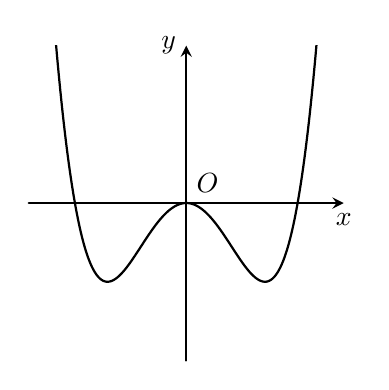
\begin{tikzpicture}[line join=round, line cap=round,>=stealth,thick,scale=1]
			\def\a{1}
			\def\b{-2}
			\def\c{0}
			\def\f(#1){\a*((#1)^4)+\b*((#1)^2)+\c}
			\def\xmin{-2}
			\def\xmax{2}
			\def\ymin{-2}
			\def\ymax{2}
			\draw[->] (\xmin,0)--(\xmax,0) node[below] { $x$};
			\draw[->] (0,\ymin)--(0,\ymax) node[left] { $y$};
			\draw (0,0) node [above right] { $O$};
			%	\foreach \x in {-3,-2,-1,1,2,3}\draw (\x,0.1)--(\x,-0.1) node [below] { $\x$};
			%	\foreach \y in {-3,-2,-1,1,2,3}\draw (0.1,\y)--(-0.1,\y) node [left] { $\y$};
			\clip (\xmin,\ymin) rectangle (\xmax,\ymax);
			\draw[thick,smooth,samples=200] plot[domain=\xmin:\xmax]  (\x,{\f(\x)});
			%			\draw (\xmax,{\f(\xmax)}) node [above right]{$x^4-2x^2+1$};
	\end{tikzpicture}}
	\loigiai{
		Đường cong trong hình vẽ là đồ thị của hàm số $ y=ax^4+bx^2+c $ với $ a>0 $ và có 3 điểm cực trị nên $ b<0 $.\\
		Trong các phương án chỉ có phương án $ y=x^4-2x^2 $ thoả mãn.
	}
\end{ex}

%%==========Câu 33
\begin{ex}%[1H3B2-3]
	Cho hình chóp $ S.ABCD $ có $ ABCD $ là hình bình hành và mặt bên $ SAB $ là tam giác vuông cân tại $ S $. Góc giữa hai đường thẳng $ SA $ và $ CD $ bằng
	\choice
	{$60^{\circ}$}
	{$90^{\circ}$}
	{$30^{\circ}$}
	{\True $45^{\circ}$}
	\loigiai{
		\immini
		{Vì tam giác $ SAB $ vuông cân tại $ S $ nên ta có $ \widehat{SAB} =45^{\circ}$.\\
		Vì $ CD \parallel AB$ nên $ \left(SA,CD\right)=\left(SA,AB\right)=\widehat{SAB}=45^{\circ}$.}
		{\begin{tikzpicture}
				\def\a{4}
				\path 	(0:0) coordinate (A)
				++(0:\a) coordinate (D)
				++(-130:\a/2) coordinate (C)
				($(A)+(C)-(D)$) coordinate (B)
				($(A)+(80:\a)$) coordinate (S)
				(intersection of A--C and B--D) coordinate (O);%giao điểm O
				\draw[dashed,thick] 	(B)--(A)--(D)	(A)--(S);
				\draw[thick] 			(B)-- (C)--(D)
				(B)--(S)	(C)--(S)	(D)--(S);
				\foreach \x/\g in {A/135,B/-135,C/-45,D/45,S/90}
				\fill[black] 	(\x) circle (1pt)
				($(\g:3mm)+(\x)$) node {$\x$};	
		\end{tikzpicture}}
	}
\end{ex}

%%==========Câu 34
\begin{ex}%[1H3K5-3]
	Cho hình chóp $S.ABCD$ có $ABCD$ là hình vuông cạnh $ a $, $ SA $ vuông góc với đáy và $ SA=a\sqrt{2} $. Khoảng cách từ $ B $ đến $ \left(SCD\right) $ bằng
	\choice
	{\True $ \dfrac{a\sqrt{6}}{3}$}
	{$\dfrac{a}{\sqrt{3}}$}
	{$a\sqrt{2}$}
	{$a$}
	\loigiai{
		\immini
		{Vì $ AB \parallel CD$ nên $ AB \parallel (SCD) $, do đó $\mathrm{d}(B,(SCD))=\mathrm{d}(A,(SCD))$\\
		Từ giả thiết ta có $ \heva{& SA \perp CD \\ & AD \perp CD} \Rightarrow CD \perp (SAD)$.\\
		Hạ $ AH \perp SD $, khi đó $ \heva{& AH \perp SD \\ & AH \perp CD} \Rightarrow AH \perp (SCD)$, do đó $\mathrm{d}(A,(SCD))=AH$\\
		Trong tam giác $ SAD $ vuông tại $ A $, đường cao $ AH $, ta có 
			\[AH=\dfrac{AS \cdot AD}{\sqrt{AS^2+AD^2}}= \dfrac{a\sqrt{6}}{3}.\]
		Vậy $\mathrm{d}(B,(SCD))=\dfrac{a\sqrt{6}}{3}$.}
		{\begin{tikzpicture}
				\def\a{4}
				\def\h{3.5}
				\path 	(0:0) coordinate (A)
				++(0:\a) coordinate (D)
				++(-130:\a/2) coordinate (C)
				($(A)+(C)-(D)$) coordinate (B)
				($(A)+(90:\h)$) coordinate (S)
				($ (S)!0.6!(D) $) coordinate (H)
				;%giao điểm O
				\draw[dashed,thick] 	(B)--(A)--(D)	(A)--(S) (A)--(H);
				\draw[thick] 			(B)-- (C)--(D)
				(B)--(S)	(C)--(S)	(D)--(S);
				\foreach \x/\g in {A/135,B/-135,C/-45,D/45,S/90,H/60}
				\fill[black] 	(\x) circle (1.5pt)
				($(\g:3mm)+(\x)$) node {$\x$};	
				\draw pic[draw,angle radius=3mm]{right angle=S--H--A};
		\end{tikzpicture}}
	}
\end{ex}

%%==========Câu 35
\begin{ex}%[2D2B3-2]
	Cho hai số thực dương $ a $ và $ b $ thoả mãn $ \ln (4a)=2\ln (a+b)-\ln b$. Mệnh đề nào dưới đây đúng?
	\choice
	{$2ab=a+b$}
	{$-2ab=a+b$}
	{$4a+b=(a+b)^2$}
	{\True $ a=b$}
	\loigiai{
		Từ giả thiết ta có 
		\allowdisplaybreaks
		\begin{eqnarray*}
			&&\ln (4a)=2\ln (a+b)-\ln b \\
			&\Leftrightarrow& \ln 4a=\ln \dfrac{(a+b)^2}{b}\\
			&\Leftrightarrow& 4ab=(a+b)^2\\
			&\Leftrightarrow& (a-b)^2=0\\
			&\Leftrightarrow& a=b.
		\end{eqnarray*}
	}
\end{ex}

%%==========Câu 36
\begin{ex}%[2H3B2-3]
	Trong KG $Oxyz$, cho hai đường thẳng $d_1\colon\heva{&x=2-t\\&y=3\\&z=-1+t}$ và $d_2\colon\heva{&x=3+t\\&y=2-t\\&z=-1}$. Mặt phẳng chứa hai đường $d_1, d_2$ có phương trình là
	\choice
	{\True$x+y+z-4=0$}
	{$x-y-z+2=0$}
	{$x+y+z+4=0$}
	{$x-y-z-2=0$}
	\loigiai{
		$d_1$ đi qua điểm $A(2;3;-1)$ và có VTCP $\overrightarrow{u}_1=(-1;0;1)$.\\
		$d_2$ đi qua điểm $B(3;2;-1)$ và có VTCP $\overrightarrow{u}_2=(1;-1;0)$.\\
		Mặt phẳng $(P)$ chứa $d_1, d_2$ có VTPT $\overrightarrow{u}_{(P)}=\left[\overrightarrow{u}_1,\overrightarrow{u}_2\right]=(1;1;1)$ và đi qua $A(2;3;-1)$.\\
		$\Rightarrow (P)\colon 1(x-2)+1(y-3)+1(z+1)=0 \Leftrightarrow x+y+z-4=0$.
	}
\end{ex}
%%==========Câu 37
\begin{ex}%[1D2B5-2]
	Một lớp học có $12$ nam và $13$ nữ. Chọn ngẫu nhiên từ lớp học đó có $5$ học sinh. Xác suất $5$ học sinh được chọn có ít nhất $1$ bạn nữ bằng
	\choice
	{$\dfrac{13}{25}$}
	{\True$\dfrac{793}{805}$}
	{$\dfrac{12}{805}$}
	{$\dfrac{12}{25}$}
	\loigiai{
		Số phần tử của không gia mẫu $n(\Omega)=\mathrm{C}_{25}^5$.\\
		Gọi $A$ là biến cố $5$ học sinh được chọn có ít nhất $1$ bạn nữ.\\
		$\Rightarrow\overline{A}$ là biến cố $5$ học sinh được không có bạn nữ.\\
		Ta có $n\left(\overline{A}\right)=\mathrm{C}_{12}^5$.\\
		$\Rightarrow P\left(\overline{A}\right)=\dfrac{\mathrm{C}_{12}^5}{\mathrm{C}_{25}^5}=\dfrac{12}{805}$.\\
		$\Rightarrow P(A)=1-P\left(\overline{A}\right)=1-\dfrac{12}{805}=\dfrac{793}{805}$.
	}
\end{ex}
%%==========Câu 38
\begin{ex}%[2D2B6-2]
	Có bao nhiêu số nguyên $x$ thỏa mãn $3\log _{8}(x+1)-\log_{2}(86-x)\geq1$?
	\choice
	{$28$}
	{$85$}
	{\True$29$}
	{$86$}
\end{ex}
\loigiai{
	Điều kiện $\heva{&x+1>0\\&86-x>0}\Leftrightarrow -1<x<86$.\\
	Ta có 
	\begin{eqnarray*}
		&&3\log _{8}(x+1)-\log _{2}(86-x)\geq1\\
		&\Leftrightarrow&3\log _{2^3}(x+1)-\log_{2}(86-x)\geq1\\
		&\Leftrightarrow&\log _{2}(x+1)-\log_{2}(86-x)\geq1\\
		&\Leftrightarrow&\log _{2}\left(\dfrac{x+1}{86-x}\right)\geq1\\
		&\Leftrightarrow&\dfrac{x+1}{86-x}\geq2\\
		&\Leftrightarrow&x+1\geq2(86-x)\quad (\text{vì}~86-x>0)\\
		&\Leftrightarrow&x\geq57.
	\end{eqnarray*}
	Kết hợp với điều kiện, ta được $57\leq x<86$.\\
	Vậy có $29$ số nguyên $x$ thỏa mãn yêu cầu bài toán.
}
%%==========Câu 39
\begin{ex}%[2D1K3-2]
	\immini{Cho hàm số $f(x)$ bậc bốn có đồ thị như hình vẽ bên.
		Có bao nhiêu số thực $m$ đế giá trị nhỏ nhất của hàm số $g(x)=f\left(x^{2}-2\right)+9 x^{2}+6mx+m^{2}+5$ bằng $4$ ?}{
		\begin{tikzpicture}[scale=0.8, font=\footnotesize, line join=round, line cap=round,>=stealth]
			\def\xmin{-4};\def\ymin{-2};\def\xmax{5};\def\ymax{4};
			\coordinate (O) at (0,0);
			\draw[->] (\xmin,0)--(\xmax,0) node[below]{$x$};
			\draw[->] (0,\ymin)--(0,\ymax) node[left]{$y$};
			\fill (O) node[below left]{$O$} circle(1pt);
			\clip ({\xmin-0.1},{\ymin-0.1}) rectangle ({\xmax+0.1},{\ymax+0.1});
			\foreach \x in {-2}{
				\fill (\x,0) node[below]{$\x$} circle(1pt);
			}
			\foreach \y in {-1,3}{
				\fill (0,\y) node[left]{$\y$} circle(1pt);
			}
			\draw (-2.88,3.52) ..controls +(0:0) 
			and +(180:0.5)..(-2,0) ..controls +(0:0.75) 
			and +(180:0.85)..(0.42,3) ..controls +(0:0.85) 
			and +(180:0.6)..(2.82,-1) ..controls +(0:0.7) 
			and +(180:0)..(3.93,3.31);
			\draw[dashed](0.42,0)--(0.42,3)--(0,3) (0,-1)--(2.82,-1)--(2.82,0);
		\end{tikzpicture}
	}
	\choice
	{$3$}
	{$1$}
	{$0$}
	{\True$2$}
\end{ex}
\loigiai{
	\begin{center}
		\begin{tikzpicture}[scale=0.8, font=\footnotesize, line join=round, line cap=round,>=stealth]
			\def\xmin{-4};\def\ymin{-2};\def\xmax{5};\def\ymax{4};
			\coordinate (O) at (0,0);
			\draw[->] (\xmin,0)--(\xmax,0) node[below]{$x$};
			\draw[->] (0,\ymin)--(0,\ymax) node[left]{$y$};
			\fill (O) node[below left]{$O$} circle(1pt);
			\clip ({\xmin-0.1},{\ymin-0.1}) rectangle ({\xmax+0.1},{\ymax+0.1});
			\foreach \x in {-3,-2,-1,1,2,3,4}{\fill (\x,0) node[below]{$\x$} circle(1pt);}
			\foreach \y in {-1,1,2,3}{\fill (0,\y) node[left]{$\y$} circle(1pt);}
			\draw (-2.88,3.52) ..controls +(0:0) and +(180:0.5)..(-2,0) ..controls +(0:0.75) and +(180:0.85)..(0.42,3) ..controls +(0:0.85) and +(180:0.6)..(2.82,-1) ..controls +(0:0.7) and +(180:0)..(3.93,3.31);
			\draw[dashed](0.42,0)--(0.42,3)--(0,3) (0,-1)--(2.82,-1)--(2.82,0)node[above]{$a$};
		\end{tikzpicture}
	\end{center}
	Có $g(x)=f\left(x^{2}-2\right)+9x^{2}+6 m x+m^{2}+5=f\left(x^{2}-2\right)+(3 x+m)^{2}+5\geq-1+0+5=4$.\\
	vì $f\left(x^{2}-2\right) \geq-1,\forall x $ và $(3 x+m)^{2} \geq 0, \forall x$.\\
	Vậy $\min _{\mathbb{R}} g(x)=4 \Leftrightarrow\heva{&f\left(x^2-2\right)=-1\\&3x+m=0}\Leftrightarrow\heva{&x^2-2=a>0\\&3x+m=0}\Leftrightarrow\hoac{&x=\sqrt{a+2};~m=-3\sqrt{a+2}\\&x=-\sqrt{a+2};~m=3\sqrt{a+2}.}$\\
	Vậy có $2$ giá trị $m$ thỏa mãn.
}
%%==========Câu 40
\begin{ex}%[2D2G6-5]
	Có bao nhiêu số nguyên $x$ sao cho ứng với mỗi $x$, tồn tại đúng 2 số thực $y$ thoả mãn
	\begin{center}
		$(1+x+y)^6\mathrm{e}^{9y-y^2}=\mathrm{e}^{2x(x+y)}$?
	\end{center}
	\choice
	{$2$}
	{$14$}
	{$11$}
	{\True$12$}
	\loigiai{
		Có $(1+x+y)^{6} \mathrm{e}^{9 y-y^{2}}=\mathrm{e}^{2 x(x+y)} \Leftrightarrow 6 \ln |1+x+y|=2 x(x+y)+y^{2}-9 y$.\\
		$\Leftrightarrow g(y)=2 x(x+y)+y^{2}-9 y-6 \ln |1+x+y|=0$.\\
		$\Rightarrow g'(y)=2 x+2 y-9-\dfrac{6}{1+x+y}=0 \Leftrightarrow x+y=5; x+y=-\dfrac{3}{2}$.\\
		Bảng biến thiên
		\begin{center}
			
\begin{tikzpicture}[scale=1, font=\normalsize]
				\tkzTabInit[nocadre=false, lgt=1.2, espcl=2, deltacl=0.6]
				{$y$/0.8,$g'(y)$/0.6,$g(y)$/2}
				{$-\infty$,$-x-1{,}5$,$-x-1$,$-x+5$,$+\infty$};
				\tkzTabLine{,-,$0$,+,d,-,$0$,+,};
				\tkzTabVar{+/$+\infty$,-/$g(-x-1{,}5)$,+D+/$+\infty$/$+\infty$,-/$g(-x+5)$,+/$+\infty$};
			\end{tikzpicture}
		\end{center}
		Phương trình có đúng 2 nghiệm khi $\hoac{&g(-x+5)=g(-x-1{,}5)=0\\&\heva{&g(-x+5)<0\\&g(-x-1{,}5)>0}\\&\heva{&g(-x+5)>0\\&g(-x-1{,}5)<0.}} (*)$ \\
		Ta có $g(-x-1,5)=\left(-\dfrac{3}{2}-x\right)^{2}-9\left(-\dfrac{3}{2}-x\right)-3 x-6\left(\dfrac{1}{2}\right) \leq 0 \Rightarrow x \in\{-5,-4\}$.\\
		Vậy $(*) \Leftrightarrow x \in\{-11, \ldots, 2\} \backslash\{-5,-4\}$. Có 12 số nguyên thoả mãn.
	}
\end{ex}

%%==========Câu 41
\begin{ex}%[2D4K5-1]
	Xét hai số phức $z$, $w$ thoả mãn $|z+2-i|=2$; $|w-z|=\sqrt{2}|w-2+i|$ và $(z-w)(\overline{z+2-i})$ là số thuần ảo. Giá trị lớn nhất của $P=\left|(w-z)(w-4-i)\right|$ bằng
	\choice
	{$56+36\sqrt{2}$}
	{$58+36\sqrt{2}$}
	{\True $72+56\sqrt{2}$}
	{$72+58\sqrt{2}$}
	\loigiai{
		Vì $|z+2-i|=2$ nên $M(z)\in(C)$ có tâm $I(-2; 1)$, $R=2$.\\
		Gọi $N(w)$ và đặt $z=a+bi$ và $w=x+yi$.\\
		Vì $(z-w)(\overline{z+2-i})=(z-w)(\overline{z-(-2+i)})$ là số thuần ảo nên $MN\perp MI$\\
		$\Leftrightarrow MN^2+MI^2=IN^2 \Leftrightarrow MN^2+R^2=IN^2$
		$\Leftrightarrow (x-a)^2+(y-b)^2+4=(x+2)^2+(y-1)^2$. \quad $(1)$\\
		Và $|w-z|=\sqrt{2}|w-2+i| \Leftrightarrow (x-a)^2+(y-b)^2=2\left[(x-2)^2+(y+1)^2\right]$. \quad $(2)$\\
		Kết hợp $(1)$, $(2)$ suy ra $2\left[(x-2)^2+(y+1)^2\right]+4=(x+2)^2+(y-1)^2 \Leftrightarrow (x-6)^2+(y+3)^2=36$.\\
		Do đó $N\in (T)$ có tâm $J(6;-3)$, $R=6$.\\
		Khi đó $P=|(w-z)(w-4-i)|=|w-z|\cdot|w-4-i|=\sqrt{2}|w-2+i|\cdot |w-4-i|=\sqrt{2}NA\cdot NB$ với $A(2;-1)$, $B(4;1)$.\\
		Ta có $JA=JB=\sqrt{20}$; $AB=2\sqrt{2}$; $JE=3\sqrt{2}$ với $E$ là trung điểm $AB$.\\
		Khi đó $NA\cdot NB\leq\dfrac{NA^2+NB^2}{2}=NE^2+\dfrac{1}{4} AB^2\leq (JE+JN)^2+\dfrac{1}{4} AB^2=(3\sqrt{2}+6)^2+2=56+36\sqrt{2}$.\\
		Do đó $\max P=72+56\sqrt{2}$.
	}
\end{ex}

%%==========Câu 42
\begin{ex}%[2D3K2-1]
	\immini
	{Cho hàm số $f(x)$ có đạo hàm liên tục trên $\mathbb{R}$ và có đồ thị như hình vẽ. Khi $\displaystyle\int\limits_{-2}^{1}\left|f(x)\right|\mathrm{d}x=50$ và $\displaystyle\int\limits_{0}^{1} f(x)\mathrm{d}x=-5$ thì $\displaystyle\int\limits_{1}^{2}\left(x^{3}+x\right) f'\left(x^{2}-3\right)\mathrm{d}x$ bằng
		\choice
		{$25$}
		{$20$}
		{$-25$}
		{\True $-20$}}
	{\begin{tikzpicture}[x=1cm,y=1cm,scale=1]
			\draw[->] (-2.5,0)--(1.5,0)node[below right]{$x$};
			\draw[->] (0,-1)--(0,2.5)node[left]{$y$};
			\fill (0,0)node[below left]{ $O$};
			\path (-2,0)coordinate[label=below left:$-2$](-2) (1,0)coordinate[label=below right:$1$](1);
			\draw[black,samples=150,smooth,domain=-2.1:1.4] plot(\x,{(\x)^3+(\x)^2-2*(\x)});
	\end{tikzpicture}}
	\loigiai{
		Đổi biến $t=x^2-3 \Rightarrow \mathrm{d}t=2 x\mathrm{d}x \Rightarrow x=1 \Rightarrow t=-2; x=2 \Rightarrow t=1$.\\
		Ta có
		\allowdisplaybreaks
		$\begin{aligned}[t]
			I&=\displaystyle\int\limits_{-2}^{1}(t+4)\cdot f'(t)\cdot \dfrac{1}{2} \mathrm{d}t=\dfrac{1}{2}\displaystyle\int\limits_{-2}^{1}(t+4) \mathrm{d}\left(f(t)\right)=\dfrac{1}{2}\left[(t+4)f(t)\bigg|_{-2}^{1}-\displaystyle\int\limits_{-2}^{1} f(t)\mathrm{d}t\right]\\
			&=\dfrac{1}{2}\left[5f(1)-2f(-2)-\displaystyle\int\limits_{-2}^{1}f(t)\mathrm{d}t\right]=-\dfrac{1}{2}\displaystyle\int\limits_{-2}^{1}f(t)\mathrm{d}t.
		\end{aligned}$\\
		Quan sát đồ thị đã cho có \[50=\displaystyle\int\limits_{-2}^{1}|f(x)|\mathrm{d}x=\displaystyle\int\limits_{-2}^{0}|f(x)|\mathrm{d}x+\displaystyle\int\limits_{0}^{1}|f(x)|\mathrm{d}x=\displaystyle\int\limits_{-2}^{0}f(x)\mathrm{d}x-\displaystyle\int\limits_{0}^{1}f(x)\mathrm{d}x=\displaystyle\int\limits_{-2}^{0} f(x)\mathrm{d}x+5 \Rightarrow \displaystyle\int\limits_{-2}^{0}f(x)\mathrm{d}x=45.\]
		Do đó $I=-\dfrac{1}{2}\displaystyle\int\limits_{-2}^{1}f(t) \mathrm{d}t=-\dfrac{1}{2}\left[\displaystyle\int\limits_{-2}^{0}f(t) \mathrm{d}t+\displaystyle\int\limits_{0}^{1}f(t) \mathrm{d}t\right]=-\dfrac{1}{2}[45-5]=-20$.
	}
\end{ex}

%%==========Câu 43
\begin{ex}%[2H2B1-2]
	Hình nón $(N)$ có đỉnh $S$, tâm đường tròn đáy là $O$, góc ở đỉnh bằng $120^{\circ}$. Một mặt phẳng qua $S$ cắt hình nón $(N)$ theo thiết diện là tam giác vuông $SAB$. Biết rằng khoảng cách giữa hai đường thẳng $AB$ và $S O$ bằng $5$. Diện tích xung quanh $S_{xq}$ của hình nón $(N)$ là
	\choice
	{\True $S_{xq}=50\pi\sqrt{3}$}
	{$S_{xq}=27\pi\sqrt{3}$}
	{$S_{xq}=36\pi\sqrt{3}$}
	{$S_{xq}=45\pi\sqrt{3}$}
\end{ex}
\loigiai{
	Góc ở đỉnh là $120^{\circ}$ nên $\widehat{OSA}=60^{\circ} \Rightarrow SA=\dfrac{OA}{\sin 60^{\circ}} \Rightarrow l=\dfrac{2}{\sqrt{3}}r$. \quad $(1)$\\
	Thiết diện là tam giác $SAB$ vuông nên vuông cân tại $S$ và $AB=SA\sqrt{2}=SB\sqrt{2}=l\sqrt{2}$.\\
	Gọi $M$ là trung điểm $AB$ thì $SO\perp OM$; $AB\perp OM$, khi đó\\
	$\mathrm{d}(SO, AB)=OM=\sqrt{OA^2-AM^2}=\sqrt{r^2-\left(\dfrac{AB}{2}\right)^2}=\sqrt{r^2-\dfrac{l^2}{2}}=5$. \quad $(2)$\\
	Từ $(1)$ và $(2)$ suy ra $r=5\sqrt{3} \Rightarrow l=10 \Rightarrow S_{xq}=\pi r l=50 \pi\sqrt{3}$.
}
%%==========Câu 44
\begin{ex}%[2H1B3-2]
	Cho khối chóp $S.ABC$ có đáy là tam giác vuông cân tại $A$. Gọi $M$ là trung điểm cạnh $BC$, hình chiếu vuông góc của $S$ lên đáy là trung điểm $I$ của $AM$. Góc giữa mặt phẳng $(SBC)$ và đáy bằng $45^{\circ}$; khoảng cách giữa hai đường thẳng $AM$ và $SB$ bằng $6$. Thể tích khối chóp đã cho bằng
	\choice
	{\True $180\sqrt{5}$}
	{$72\sqrt{2}$}
	{$108\sqrt{3}$}
	{$468\sqrt{13}$}
	\loigiai{
		Đặt $AB=AC=x,\,\,(x>0) \Rightarrow BC=x\sqrt{2}$.\\
		Có $\heva{&BC\perp AM\\&BC\perp SI} \Rightarrow BC\perp (SAI) \Rightarrow \left((SBC),(ABC)\right)=\widehat{SMI}=45^{\circ} \Rightarrow SI=IM=\dfrac{AM}{2}=\dfrac{BC}{4}=\dfrac{x\sqrt{2}}{4}$.\\
		Dựng hình bình hành $IMBH$.\\
		Khi đó $AM\parallel BH \Rightarrow AM \parallel (SBH) \Rightarrow \mathrm{d}(AM, SB)=\mathrm{d}(AM,(SBH))=\mathrm{d}(I,(SBH))$.\\
		Ta có $IM\perp BC \Rightarrow IH\perp BH$ kẻ $IK\perp SH \Rightarrow IK\perp(SBH)$.\\
		Có $\dfrac{1}{IK^2}=\dfrac{1}{IS^2}+\dfrac{1}{IH^2} \Rightarrow\dfrac{1}{6^2}=\dfrac{1}{\left(\dfrac{x\sqrt{2}}{4}\right)^2}+\dfrac{1}{\left(\dfrac{x\sqrt{2}}{2}\right)^2} \Rightarrow x=6\sqrt{10}$.\\
		Vậy $V_{S.ABC}=\dfrac{1}{3} S_{ABC}\cdot SI=\dfrac{1}{3}\cdot\dfrac{1}{2}\cdot x\cdot x\cdot\dfrac{x\sqrt{2}}{4}=\dfrac{x^3\sqrt{2}}{24}=\dfrac{\sqrt{2}(6\sqrt{10})^3}{24}=180\sqrt{5}$.
	}
\end{ex}

%%==========Câu 45
\begin{ex}%[2D2K6-5]
	Xét hai số thực $a$, $b$ thỏa mãn $a^2+b^2=6a+8b-24$ và hai số thực không âm $x$ và $y$ thỏa mãn\\ $4x+y\cdot 2^{\sqrt{2x+2y+1}}\leq 6$. Tổng giá trị lớn nhất và giá trị nhỏ nhất của biểu thức $P=(a-x)^2+(b-y)^2$ bằng
	\choice
	{$\dfrac{20+11\sqrt{2}}{4}$}
	{$\dfrac{321}{8}$}
	{\True $\dfrac{417-44\sqrt{2}}{8}$}
	{$\dfrac{209-4\sqrt{61}}{4}$}
	\loigiai{
		\begin{center}
			\begin{tikzpicture}[scale=1, font=\footnotesize, line join=round, line cap=round,>=stealth]
				\def\xmin{-2};\def\ymin{-3};\def\xmax{6};\def\ymax{5};
				\coordinate (O) at (0,0);
				\coordinate (A) at (1.5,0);
				\coordinate (B) at (0,1.5);
				\coordinate (I) at (3,4);
				\coordinate (M) at ($(I)!1!-10:(4,4)$);
				\coordinate (N) at (0.8,0.2);
				\path[name path=dtron] (I) circle(1 cm);
				\path[name path=dthangio] (I) -- (O);
				\path[name intersections={of=dtron and dthangio }]
				(intersection-1) coordinate (Q);
				\coordinate (M_2) at ($(I)+1*(I)-1*(Q)$);
				\coordinate (C) at ($(A)!(I)!(B)$);
				\path[name path=dtron] (I) circle(1 cm);
				\path[name path=dthangic] (I) -- (C);
				\path[name intersections={of=dtron and dthangic }]
				(intersection-1) coordinate (M_1);
				\fill[cyan!50] (0,0)--(1.5,0)--(0,1.5)--cycle;
				\draw[->] (\xmin,0)--(\xmax,0) node[below]{$x$};
				\draw[->] (0,\ymin)--(0,\ymax) node[left]{$y$};
				\fill (O) node[below left]{$O$} circle(1pt);
				\clip ({\xmin-0.1},{\ymin-0.1}) rectangle ({\xmax+0.1},{\ymax+0.1});
				\foreach \x in {-1,1,2,3,4,5}{
					\fill (\x,0) node[below]{$\x$} circle(1pt);}
				\foreach \y in {-2,-1,1,2,3,4}{
					\fill (0,\y) node[left]{$\y$} circle(1pt);}
				\draw[samples=100] plot[domain=-1.5:3](\x,{-\x+1.5}) node[right] {$2x+2y-3=0$};
				\draw(I) circle(1 cm) (M)--(N);
				\draw [dashed] (O)--(M_2) (I)--(C);
				\draw[black] pic[draw, angle radius=2mm, angle eccentricity=1.5]{right angle=A--C--I};
				\foreach \t/\g in {I/90,M/-10,N/180,M_2/45,C/-90,M_1/170}{\draw[fill=white] (\t) circle (1pt) node[shift={(\g:7pt)},font=\scriptsize]{$\t$};}
			\end{tikzpicture}
		\end{center}
		Ta có $a^2+b^2=6a+8b-24\Leftrightarrow (a-3)^2+(b-4)^2=1 \Rightarrow M(a;b) \in (C)$ có tâm $I(3;4)$, $R=1$.\\
		Xét $4x+y\cdot 2^{\sqrt{2x+2y+1}}\leq 6$. Đặt $t=\sqrt{2x+2y+1},(t\geq 1,\forall x,y\geq 0) \Rightarrow 2x+2y+1=t^2\Rightarrow 2x=t^2-2y-1$.\\
		Bất phương trình trở thành $g(t)=2(t^2-2y-1)+y\cdot 2^t-6 \leq 0 ~ (*)$.\\
		Có $g'(t)=4t+y\cdot 2^t \ln 2 \geq 4\cdot 1+0=4,\forall t \geq 1 \Rightarrow g(t)$ đồng biến trên $[1;+\infty)$ và nhận thấy\\ $g(2)=0 \Rightarrow (*)\Leftrightarrow g(t)\leq g(2)\Leftrightarrow t\leq 2 \Leftrightarrow 2x+2y+1\leq 4 \Leftrightarrow 2x+2y-3 \leq 0$.\\
		Do đó điểm $N(x;y)$ thỏa mãn $x\geq 0,y\geq 0,2x+2y-3\leq 0$ là tam giác vuông $OAB$ với $A\left(\dfrac{3}{2};0\right)$ và $B\left(0;\dfrac{3}{2}\right)$.\\
		Khi đó $P=(a-x)^2+(b-y)^2=MN^2$ và \\
		$MN\geq IN-IM=IN-R=IN-1\geq \mathrm{d}(I,d)-1=\dfrac{11}{2\sqrt{2}}-1$. Dấu bằng xảy ra khi $M$ trùng $M_1$, $N$ trùng $C$.\\
		Và $MN\leq IN+IM =IN+R=IN+1 \leq \max\{IO,IA,IB\}+1=\max \{5,\dfrac{\sqrt{73}}{2},\dfrac{\sqrt{61}}{2} \}+1=5+1=6$.\\
		Dấu bằng xảy ra khi $M$ trùng $M_2$, $N$ trùng $O$.\\
		Vậy $\max P+\min P=6^2+\left(\dfrac{11}{2\sqrt{2}}-1 \right)^2=\dfrac{417-44\sqrt{2}}{8}$.
	}
\end{ex}

%%==========Câu 46
\begin{ex}%[2H3K2-8]
	Trong KG $Oxyz$, cho hai điểm $A(2;1;0)$, $B(1;2;0)$ và điểm $M$ di động trên tia $Oz$. Gọi $H$, $K$ lần lượt là hình chiếu vuông góc của $A$ lên $OB$ và $MB$. Đường thẳng $HK$ cắt trục $Oz$ tại điểm $N$. Khi thể tích khối tứ diện $ABMN$ nhỏ nhất thì mặt phẳng $(AHK)$ có dạng $ax+by+cz-4=0$. Giá trị của $a+b+c$ bằng
	\choice
	{$-1$}
	{$5$}
	{\True $1$}
	{$-4$}
	\loigiai{
		\immini
		{Ta có $A(2;1;0)$, $B(1;2;0)$ $\Rightarrow A,~ B \in (Oxy)$.\\
		Có $\heva{&AK\perp MB\\&AH\perp OB;~AH\perp OM \Rightarrow AH \perp (OBM) \Rightarrow AH \perp MB}$\\
		$\Rightarrow MB \perp (AHK)$.\\
		Gọi $M(0;0;m)$, $(m>0)$ thuộc tia $Oz$ khi đó $\overrightarrow{MB}=(1;2;-m)$\\
		$\Rightarrow (AHK)\colon 1(x-2)+2(y-1)-mz=0$.\\
		$\Rightarrow N=HK \cap Oz =(AHK) \cap Oz \Rightarrow N\left(0;0;-\dfrac{4}{m}\right)$.\\
		Ta có
		\allowdisplaybreaks
		$\begin{aligned}[t]
			V_{ABMN}&=V_{M.OAB}+V_{N.OAB}=\dfrac{1}{3}S_{OAB}\cdot OM +\dfrac{1}{3}S_{OAB}\cdot ON\\
			&=\dfrac{1}{3}S_{OAB}(OM+ON)=\dfrac{1}{3}S_{OAB}\cdot MN
		\end{aligned}$\\
		Vậy $V_{ABMN}$ nhỏ nhất khi $MN$ nhỏ nhất.\\
		Ta có $MN=m+\dfrac{4}{m}\geq 2\sqrt{m\cdot \dfrac{4}{m}}=4$.\\
		Dấu bằng xảy ra khi $m=\dfrac{4}{m}\Rightarrow m=2$.\\
		Vậy $(AHK)\colon x+2y-2z-4=0 \Rightarrow a+b+c=1+2-2=1$.}
		{\begin{tikzpicture}[scale=1.5, font=\footnotesize, line join=round, line cap=round,>=stealth]
				\def\xmin{-2};\def\ymin{-3};\def\xmax{6};\def\ymax{5};
				\coordinate (O) at (0,0);
				\coordinate (B) at (2,-1);
				\coordinate (A) at (3,0);
				\coordinate (M) at (0,2);
				\coordinate (K) at ($(M)+2/5*(B)-2/5*(M)$);
				\coordinate (H) at ($(O)+1/4*(B)-1/4*(O)$);
				\coordinate (N) at (intersection of M--O and K--H);
				\draw (A)--(B)--(O)--(M)--cycle (M)--(B) (A)--(K)--(N)--(O);
				\draw [dashed] (O)--(A)--(H) (A)--(N);
				\draw[black] pic[draw, angle radius=2mm, angle eccentricity=1.5]{right angle=B--K--A};
				\draw[black] pic[draw, angle radius=2mm, angle eccentricity=1.5]{right angle=B--H--A};
				\foreach \t/\g in {O/180,B/-90,A/0,M/70,K/90,H/200,N/-90}{\draw[fill=white] (\t) circle (1pt) node[shift={(\g:7pt)},font=\scriptsize]{$\t$};}
		\end{tikzpicture}}
	}
\end{ex}

%%==========Câu 47
\begin{ex}%[2D3K3-1]
	Cho hàm số $f(x)=2x^3+ax^2+bx+c$ có hai điểm cực trị là $x_1$, $x_2$ sao cho $f(x_2)=f(x_1)+64$. Gọi $y=g(x)$ là đường thẳng qua hai điểm cực trị của đồ thị hàm số $f(x)$. Diện tích hình phẳng giới hạn bởi hai đường $y=f(x)$ và $y=g(x)$ bằng
	\choice
	{$8$}
	{\True $16$}
	{$24$}
	{$32$}
	\loigiai{
		Đặt $x_1=m$, $x_2=n \Rightarrow f(n)-f(m)=64$ và khi đó $f'(x)=6x^2+2ax+b=6(x-m)(x-n)$.\\
		Ta có $f(n)-f(m)=\displaystyle \int\limits_{m}^n6(x-m)(x-n)\mathrm{\,d}x=(m-n)^3=64\Rightarrow m-n=4$.\\
		Đường thẳng qua hai điểm cực trị của đồ thị hàm bậc ba sẽ cắt đồ thị tại điểm thứ ba là điểm uốn của đồ thị hàm bậc ba và là trung điểm của đoạn thẳng nối hai điểm cực trị.\\
		Vậy $f(x)-g(x)=2(x-m)(x-n)\left(x-\dfrac{m+n}{2}\right)$.\\
		Suy ra $S=\displaystyle \int\limits_{n}^m \left| 2(x-m)(x-n)\left(x-\dfrac{m+n}{2}\right)  \right|\mathrm{\,d}x=\dfrac{1}{16}(m-n)^4=\dfrac{1}{16}\cdot 4^4=16$.\\
		\textbf{Chú ý:} Bước tính $S$ các em chọn tùy ý chẳng hạn $m=4$; $n=0$ $\Rightarrow S= \displaystyle \int\limits_{0}^4 \left| 2(x-4)(x-0)\left(x-\dfrac{4+0}{2}\right)  \right|\mathrm{\,d}x=16$.
		
	}
\end{ex}

%%==========Câu 48
\begin{ex}%[Dự án text đề Vted 2023]%[Huỳnh Xuân Tín]%[2H3G3-8] 
	Trong không gian $O x y z$, cho mặt cầu $(S)\colon (x-4)^2+(y+3)^2+(z+6)^2=42$. Có bao nhiêu điểm $M$ thuộc mặt phẳng $(O x y)$, với toạ độ là các số nguyên, mà từ $M$ kẻ được đến $(S)$ hai tiếp tuyến vuông góc với nhau và cùng vuông góc với trục hoành?
	\choice
	{$13$}
	{$9$}
	{\True $4$}
	{$8$}
	\loigiai{
		Mặt cầu đã cho có tâm $I(4 ;-3 ;-6), R=\sqrt{42}$.\\
		Gọi $M(a ; b ; 0) \in(O x y)$, $(a, b \in \mathbb{Z})$. Gọi hai tiếp tuyến thoả mãn là $M A, M B$ với $A, B$ là các tiếp điểm.\\
		Vì $M A \perp O x ; M B \perp O x \Rightarrow(M A B) \perp O x \Rightarrow(M A B)\colon x-a=0$.\\
		Khi đó $(M A B) \cap(S)=(C)$ có tâm $H$ là hình chiếu của $I$ lên  $(M A B)$; $R_{(C)}=\sqrt{R^2-\mathrm{d}^2(I,(M A B))}$ và $M A, M B$ là tiếp tuyến kẻ từ $M$ đến $(C)$.
		\begin{center}
			\begin{tikzpicture}[scale=0.7,>=stealth, font=\footnotesize, line join=round, line cap=round]
				%	\draw[color=gray!50,dashed] (-6,-6) grid (6,6);
				%	\draw[->] (-6,0)--(6,0) node [below]{$x$};
				%	\draw[->] (0,-6)--(0,6) node [left]{$y$};
				%	\clip (-6,-6) rectangle (6,6);
				%%%%%%%%%%%%%%%
				\tkzDefPoints{0/0/A,5/0/H,5/5/B,0/5/M}
				\tkzDrawSegments(A,M A,H H,B B,M M,H)
				\tkzDrawCircle[radius](H,A)
				\tkzDrawPoints[fill=black](A,B,M,H)
				\tkzLabelPoints[below](H)
				\tkzLabelPoints[above](M,B)
				\tkzLabelPoints[left](A)
			\end{tikzpicture}
		\end{center}
		\noindent Vì $M A \perp M B \Rightarrow M A H B$ là hình vuông nên $M A=\dfrac{M H}{\sqrt{2}}$.\\
		Khi đó $MAHB$ là hình vuông tâm $I$.\\
		Suy ra
		\allowdisplaybreaks
		$\begin{aligned}[t]
			MI^2&=M A^2+A I^2=M A^2+R^2=\dfrac{M H^2}{2}+R^2\\
			&=\dfrac{M I^2-I H^2}{2}+R^2=\dfrac{M I^2-\mathrm{d}^2(I,(M A B))}{2}+R^2
		\end{aligned}$\\
		$\Leftrightarrow M I^2=2 R^2-\mathrm{d}^2(I,(M A B))\\ \Leftrightarrow (a-4)^2+(b+3)^2+6^2=84-(a-4)^2
		\Leftrightarrow 2(a-4)^2+(b+3)^2=48 $
		Vì $a,b\in \mathbb{Z}$ nên $2(a-4)^2\le 48\Leftrightarrow(a-4)^2\le 24\Rightarrow (a-4)^2\in\{0;1;4;9;16\}\Rightarrow a\in\{0;1;2;3;4;5;6;7;8\}$.\\
		Thay vào ta suy ra $(a ; b)=(0 ;-7) ;(0 ; 1) ;(8 ;-7) ;(8 ; 1)$. 
	}
\end{ex}

%%==========Câu 49
\begin{ex}%[Dự án text đề Vted 2023]%[Huỳnh Xuân Tín]%[2D4G4-1]
	Trên tập số phức, xét phương trình $z^2+2 m z+n^2+5=0$ (với $m$, $n$ là tham số thực). Có bao nhiêu cặp số $(m ; n)$ để phương trình đã cho có hai nghiệm phức $z_1$, $z_2$ sao cho các điểm biểu diễn của $z_1$, $z_2$, $z_3=1$, $z_4=5$ là bốn đỉnh của một hình vuông?
	\choice
	{$4$}
	{\True $2$}
	{$3$}
	{$1$}
	\loigiai{
		Xét $\Delta'=m^2-n^2-5$.
		\begin{enumerate}[TH 1.]
			\item Nếu $\Delta' \geq 0 \Rightarrow A\left(z_1\right), B\left(z_2\right), C\left(z_3\right), D\left(z_4\right) \in O x$ không tạo thành hình vuông.
			\item 
			\immini
			{Nếu $\Delta'<0 \Rightarrow z_1=-m-\sqrt{n^2+5-m^2} \cdot i$; $z_2=-m+\sqrt{n^2+5-m^2} \cdot i$.\\
			Khi đó $A\left(-m ;-\sqrt{n^2+5-m^2}\right)$, $B\left(-m ; \sqrt{n^2+5-m^2}\right)$, $C(1 ; 0)$, $D(5 ; 0)$.\\
			Ta có $C, D \in O x ; A, B \in d: x=-m$ đối xứng với nhau qua trục hoành. Do đó hình vuông tạo bởi bốn điểm này nếu có là $A C B D$.\\
			Trước tiên $A B \cap C D=I(-m ; 0) \equiv I(3 ; 0) \Rightarrow m=-3$ (tại trung điễm mỗi đường). Khi đó rõ ràng $A C B D$ là một hình thoi.\\
			Vậy để là hình vuông thì cần thêm điều kiện $A B=C D=4 \Leftrightarrow 2 \sqrt{n^2+5-m^2}=4$ kết hợp với $m=-3 \Rightarrow(m ; n)=\left( -3 ;-2 \sqrt{2}\right)$; $\left( -3 ; 2 \sqrt{2}\right)$.}
			{\begin{tikzpicture}[scale=0.8,>=stealth, font=\footnotesize, line join=round, line cap=round]
					%	\draw[color=gray!50,dashed] (-6,-6) grid (6,6);
					\draw[->] (-1,0)--(6,0) node [below]{$x$};
					\draw[->] (0,-3)--(0,3) node [left]{$y$};	
					\tkzDefPoints{3/-2/A,3/2/B,1/0/C,5/0/D,3/0/I}
					\tkzDrawSegments(A,B B,C C,A A,D D,B)
					\tkzDrawPoints[fill=black](A,B,C,D,I)
					\tkzLabelPoints[below](A,C,D)
					\tkzLabelPoints[above](B)
					\tkzLabelPoints[below right](I)
				\end{tikzpicture}}
		\end{enumerate}
		
	}
\end{ex}

%%==========Câu 50
\begin{ex}%[Dự án text đề Vted 2023]%[Huỳnh Xuân Tín]%[2D1G2-2]
	\immini{Cho hàm số $ y=f(x) $ có đạo hàm và liên tục trên $ \mathbb{R} $ và $ f(0)=0 $. Biết hàm số $ y=f'(x) $ có đồ thị như hình vẽ. 
		Số điểm cực tiểu của hàm số $ g(x)=\left\vert f(x^2)-2x\right\vert $ là
		\choice
		{\True $ 2$}
		{$1$}
		{$3$}
		{$0$}}{\begin{tikzpicture}[scale=.5, font=\footnotesize, line join=round, line cap=round,>=stealth]
			\def\a{-1/2}  
			\def\xmin{-1.5} \def\xmax{5.3}
			\def\ymin{-1.5} \def\ymax{6} 
			\draw[->] (\xmin,0)--(\xmax,0) node [below]{$x$};
			\draw[->] (0,\ymin)--(0,\ymax) node [left]{$y$};
			\node at (0,0) [below left]{$O$};
			%	\draw[fill=black](4,0)circle (.5pt) node[below ]{\footnotesize $4$};
			%	\draw[fill=black](2,0)circle (.5pt) node[below]{\footnotesize $2$};
			\draw[fill=black](1,0)circle (.5pt) node[below ]{\footnotesize $1$};
			\draw[fill=black](0,1)circle (.5pt) node[left]{\footnotesize $1$};
			%	\draw[fill=black](0,3)circle (.5pt) node[left]{\footnotesize $3$};
			%	\draw[fill=black](0,5)circle (.5pt) node[left]{\footnotesize $5$};
			\clip (\xmin+0.1,\ymin+0.1) rectangle (\xmax-0.1,\ymax-0.1);
			\draw
			($(-.5,-.3)-(90:8)$)--
			(0,0) .. controls +(0:0) and +(180:0.5) ..
			(1,3) .. controls +(0:0.5) and +(180:0.25) ..
			(2,1) .. controls +(0:0.5) and +(180:0) ..
			(4,5) --($(4.2,5.4)+(75:3.2)$);
			\draw[dashed] (1,0) |- (1,3) |- (0,3);
			\draw[dashed] (2,0) |- (2,1) |- (0,1);
			%	\draw[dashed] (4,0) |- (4,5) |- (0,5);
			\fill (1,3) circle(1pt); \fill (2,1) circle(1pt); \fill (0,0) circle(1pt); \fill (4,5) circle(1pt);
	\end{tikzpicture}}	
	\loigiai{
		Xét $ h(x)= f(x^2)-2x$.\\
		Ta có $ h'(x)=2xf'(x^2)-2=2\left(xf'(x^2)-1\right) $.
		\begin{itemize}
			\item Dễ thấy $x=0$ không phải là nghiệm phương trình $h'(x)=0 $.
			\item Xét $x\ne 0$, ta có 
			\[h'(x)=0 \Leftrightarrow  xf'(x^2)-1=0\Leftrightarrow f'(x^2)=\dfrac{1}{x}. \qquad(*)\]
			Đặt $t=x^2 \Leftrightarrow \hoac{&x=\sqrt{t} \\ &x=-\sqrt{t}}$. Khi đó, $(*)$ trở thành $\hoac{&f'(t)=\dfrac{1}{\sqrt{t}} \\ &f'(t)=\dfrac{-1}{\sqrt{t}}.}$
		\end{itemize}	
		Vẽ chung đồ thị ba hàm số $y=f'(x)$, $y=\dfrac{1}{\sqrt{x}}$ và $y=\dfrac{-1}{\sqrt{x}}$ trên cùng hệ tọa độ $Oxy$. 
		\begin{center}
			\begin{tikzpicture}[scale=.5, font=\footnotesize, line join=round, line cap=round,>=stealth]
				\def\a{-1/2}  
				\def\xmin{-1.5} \def\xmax{5.3}
				\def\ymin{-2.5} \def\ymax{6} 
				\draw[->] (\xmin,0)--(\xmax,0) node [below]{$x$};
				\draw[->] (0,\ymin)--(0,\ymax) node [left]{$y$};
				\node at (0,0) [below left]{$O$};
				%	\draw[fill=black](4,0)circle (.5pt) node[below ]{\footnotesize $4$};
				%	\draw[fill=black](2,0)circle (.5pt) node[below]{\footnotesize $2$};
				\draw[fill=black](1,0)circle (.5pt) node[below ]{\footnotesize $1$};
				\draw[fill=black](0,1)circle (.5pt) node[left]{\footnotesize $1$};
				%	\draw[fill=black](0,3)circle (.5pt) node[left]{\footnotesize $3$};
				%	\draw[fill=black](0,5)circle (.5pt) node[left]{\footnotesize $5$};
				\clip (\xmin+0.1,\ymin+0.1) rectangle (\xmax-0.1,\ymax-0.1);
				\draw
				($(-.5,-.3)-(90:8)$)--
				(0,0) .. controls +(0:0) and +(180:0.5) ..
				(1,3) .. controls +(0:0.5) and +(180:0.25) ..
				(2,1) .. controls +(0:0.5) and +(180:0) ..
				(4,5) --($(4.2,5.4)+(75:3.2)$);
				\draw[dashed] (1,0) |- (1,3) |- (0,3);
				\draw[dashed] (2,0) |- (2,1) |- (0,1);
				%	\draw[dashed] (4,0) |- (4,5) |- (0,5);
				\draw[smooth,samples=200,domain=0.01:\xmax] plot(\x,{1/(sqrt(\x))}) node[above left]{$y=\dfrac{1}{\sqrt{x}}$}; 
				\draw[smooth,samples=200,domain=0.01:\xmax] plot(\x,{-1/(sqrt(\x))}) node[below left]{$y=\dfrac{-1}{\sqrt{x}}$}; 
				\fill (1,3) circle(1pt); \fill (2,1) circle(1pt); \fill (0,0) circle(1pt); \fill (4,5) circle(1pt);
			\end{tikzpicture}
		\end{center}
		Từ đồ thị, ta thấy phương trình $f'(t)=\dfrac{1}{\sqrt{t}}$ có $1$ nghiệm duy nhất $ t=t_0\in(0;1) $;	\\
		phương trình $f'(t)=-\dfrac{1}{\sqrt{t}}$ vô nghiệm.\\
		Suy ra phương trình $ h'(x)=0 $ có $ 1 $ nghiệm $ x=\sqrt{t_0} $.
		\begin{center}
			\begin{tikzpicture}[scale=1, >=stealth]
				\tkzTabInit[nocadre=false, lgt=1.2, espcl=2.5, deltacl=1.5]{$x$/0.6, $h'(x)$/0.6, $h(x)$/3}{$-\infty$, $0$, $\sqrt{t_0}$, $$, $2$,  $+\infty$}
				\tkzTabLine{,-,, -, 0,+, ,,  ,+, } 
				\draw
				(N12)++(0,-0.8)node[](A){$$}
				(N22)++(0,-1.5)node[](B){$$}
				(N31)++(0,-2.75)node[](C){$h(\sqrt{t_0})$}
				(N42)++(0,-1.5)node[](D){$$}
				(N62)++(0,-0.5)node[](E){$+\infty$}
				(N12)++(0,-1.6)node[above](G){}
				(N62)++(0,-1.6)node[above](H){}
				;
				\draw[->](A)--(B);
				\draw[->](B)--(C);
				\draw[->](C)--(D);
				\draw[->](D)--(E);
				\draw(G)--(H)+(0.7,0)node[]{$y=0$};
				\draw[dashed](N21)--($(N22)!.5!(N23)$);
				\draw[dashed](N51)--($(N52)!.3!(N53)$);
			\end{tikzpicture}
		\end{center}
		Ta có $ h(0)=f(0)=0 $.\\
		Từ bảng biến thiên của hàm số $ h(x) $ suy ra hàm số $ y=\vert h(x)\vert $ có hai điểm cực tiểu.
	}
\end{ex}




\Closesolutionfile{ans}
\inputansbox{10}{ans/ans-Vted-16-2023}